\chapter{典型光学系统}

\begin{introduction}
	\item 眼睛(第 \ref{sect:eye} 节)
	\item 放大镜(第 \ref{sect:magnifier} 节)
	\item 显微镜系统(第 \ref{sect:microscope} 节)
	\item 望远镜系统(第 \ref{sect:telescope} 节)
\end{introduction}

\section{眼睛}
\label{sect:eye}
\subsection{眼睛的构造}

\begin{figure}[htbp]
	\centering
	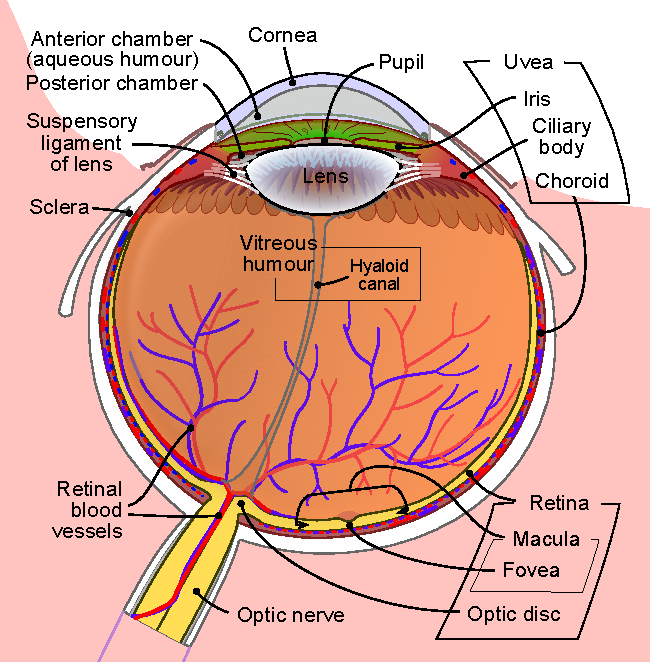
\includegraphics[width=0.5\textwidth]{structure-of-eye.pdf}
	\caption{人眼的内部构造}
	\label{fig:structure-of-eye}
\end{figure}

人眼呈球状,直径约$25\mathrm{mm}$,右眼的内部构造如\figref{fig:structure-of-eye} 所示。

眼球被一层坚韧的膜包围,前面突出的透明部分为\textbf{角膜},其余部分为\textbf{巩膜}。角膜后是充满折射率为$1.336$的透明液体的前室,前室的后壁为\textbf{虹彩膜},其中央部分有一圆孔,为\textbf{瞳孔}。虹膜之后是\textbf{水晶体},它是由多层薄膜构成的双凸透镜,各层折射率不同,内层约为$1.41$,外层约为$1.38$。水晶体后面是后室,也称为眼腔,内部充满折射率为$1.336$的透明胶装液体,称\textbf{玻状液}。后室的内壁与玻状液紧贴的部分是由视神经末梢组成的膜,称为\textbf{视膜},是眼球系统所成像的接收器,共有十层结构,前八层对光透明但不引起刺激,第九层是感光层,布满视神经细胞。第十层与脉络膜相连。\textbf{脉络膜}是网膜外包围着的一层黑色膜,吸收透过网膜的光线,避免感光器官受到强光的刺激。在视神经进入眼腔处附近的网膜上,有一个椭圆形区域,该区域内没有感光细胞,不产生视觉,称为\textbf{盲斑}。距盲斑中心$15^{\circ}30'$,在太阳穴方向有一椭圆区域e,大小为$1\mathrm{mm}$(水平方向)$\times0.8\mathrm{mm}$(垂直方向),称为\textbf{黄斑}。在黄斑中心有一$0.3\mathrm{mm}\times0.2\mathrm{mm}$的凹部,称为\textbf{中心凹}。中心凹密集了大量的感光细胞,是网膜上视觉最灵敏的区域。当眼睛观察外界物体时,会本能地转动眼球,使像成在中心凹上。因而称通过眼睛节点和中心凹的直线为眼睛的\textbf{视轴}。\footnote{本段对于眼睛结构的描述仅为简单的介绍,如需进一步了解请查阅相关文献。}

\begin{definition}{标准眼}{standard-eye}
	眼睛作为一个光学系统,其有关参数可由专门的仪器测出。根据大量的测量结果,定出了眼睛的各项光学常数,包括角膜、水状液、波状液和水晶体的折射率、各光学表面的曲率半径,以及各有关距离。满足这些光学常数值的眼睛称为标准眼。
\end{definition}

\begin{definition}{简约眼}{reduced-eye}
	为了作近似计算方便,可把标准眼简化为一个折射球面的模型,称为简约眼。简约眼的有关参数如下所示:
	\begin{enumerate}
		\item 折射面的曲率半径:$5.56\mathrm{mm}$
		\item 像方介质的折射率:$4/3=1.333$
		\item 视网膜的曲率半径:$9.7\mathrm{mm}$
	\end{enumerate}
	可算得简约眼的物方焦距为$-16.70\mathrm{mm}$,像方焦距为$22.26\mathrm{mm}$,光焦度为$59.88$屈光度。
\end{definition}

\subsection{眼睛的调节}
水晶体在睫状肌的作用下曲率可变,使不同远近的物体精确地成像在网膜上。当肌肉收缩时,水晶体曲率变大,可看清近物;肌肉放松时,水晶体曲率变小,可看清远物。眼睛的这种本能地改变水晶体光焦度以看清不同远近物体的功能称为\textbf{调节}。当肌肉完全放松时,眼睛所能看清的最远的点称为\textbf{远点};当肌肉收缩到最紧张状态时所能看清的最近点称为\textbf{近点}。分别以$p$和$r$表示近点和远点到眼睛物方主点的距离,则其倒数$P=1/p$和$R=1/r$就是近点和远点会聚度和屈光度数。二者之差以$A$表示,即
\begin{equation}
A=R-P
\end{equation}
称为调节范围或调节能力。

\subsubsection{正常眼}
正常眼的调节范围随年龄的变化而变化,年龄增大,肌肉收缩功能衰退,近点逐渐移远,调节范围减小。

\begin{definition}{明视距离}{distance-of-distinct-vision}
	明视距离是指正常眼在正常照明(约$50\mathrm{lx}$)下的正常阅读距离,国际规定为$250\mathrm{mm}$。
\end{definition}


\subsubsection{非正常眼}
非正常眼主要有以下几种:
\begin{enumerate}
	\item \textbf{近视眼}:远点在眼前的有限远处,$R<0$,眼球偏长,像方焦点位于网膜前,只有有限远处的物体才能成像在网膜上。\uline{校正方法:负光焦度眼镜}。
	\item \textbf{远视眼}:远点在眼镜之后,$R>0$,眼球偏短,像方焦点位于网膜后,只有会聚光束才能聚焦到网膜上。\uline{校正方法:正光焦度眼镜}。
	\item \textbf{散光眼}和\textbf{斜视眼}:水晶体位置不正、各个折射面曲率不正常或不对称。\uline{校正方法:前者用柱面透镜,后者用光楔}。
	\item \textbf{近视散光}:同时存在多种缺陷。
\end{enumerate}

\subsection{眼睛的适应}
人眼除了能随物体距离的改变而调节水晶体的曲率外,还能在不同亮暗条件下工作。眼睛所能感受到的光亮度变化范围为$10^{12}:1$。人从亮出到暗处发生暗适应,从暗处到亮处发生亮适应。

\subsection{眼睛的分辨率}
眼睛能分辨开两个很靠近的点的能力称为眼睛的\textbf{分辨率}。刚能分辨开的两个点对眼睛物方节点的张角称为眼睛的\textbf{极限分辨角}。分辨率与极限分辨角成反比。

入瞳为$D$的理想光学系统,其极限分辨角为
\begin{equation}
\varphi=\frac{1.22\lambda}{D}
\label{eq:limiting-angle-of-resolution}
\end{equation}
对$555$纳米的色光而言,若入瞳单位取毫米,将极限分辨角的单位取作秒,则有
\begin{equation}
\varphi''=\frac{140}{D}
\end{equation}

\begin{note}
	影响分辨率的因素:
	\begin{enumerate}
		\item 眼睛的分辨率随被观察物体的亮度和对比度而异。对比度一定,亮度越大分辨率越高;亮度一定,对比度越大分辨率越高。
		\item 照明光的光谱是影响分辨率的一个重要因素,由于眼睛有较大的色差,单色光的分辨率要比白光高,并以$555$nm的黄绿光为最高。
		\item 网膜上成像位置对分辨率有一定的影响,成像处于黄斑处分辨率最高。
	\end{enumerate}
\end{note}

\subsection{眼睛的瞄准精度}
在很多测量工作中,为了读数,常用某种标志对目标物进行对准或重合,例如用一根直线与另一直线重合。这种重合或对准的过程为\textbf{瞄准}。由于受到人眼分辨率的限制,二者完全重合是不可能的。偏离于完全重合的程度称为\textbf{瞄准精度}。瞄准精度随所选取的瞄准标志而异,最高时可达人眼分辨率的$1/5\sim1/10$。

\subsection{眼睛的立体视觉}
眼睛观察空间物体时,能区别它们的相对远近而具有立体视觉。通常,人们总以双眼观物。物在两眼中各自成像,两眼的视觉汇合到大脑产生但因的印象。物在两眼网膜上的像必须位于网膜的对应点,即相对于黄斑中心的同一侧,才有单像的印象。

\begin{figure}[htbp]
	\centering
	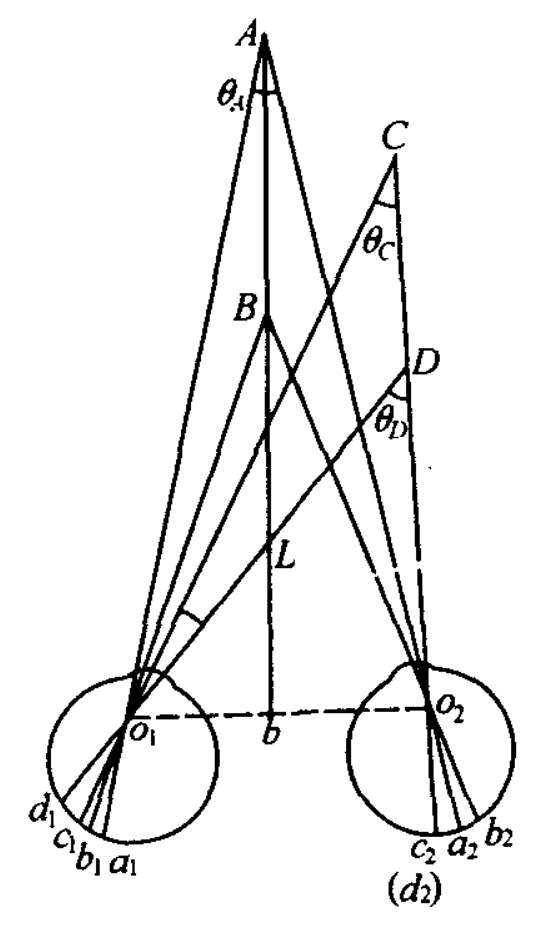
\includegraphics[width=0.3\textwidth]{two-eyes.png}
	\caption{双眼立体视觉}
	\label{fig:two-eyes}
\end{figure}

如\figref{fig:two-eyes} 所示,当两眼注视$A$点时,$A$点的像$a_1$和$a_2$位于黄斑中心,较近的B点在两网膜上的像$b_1$和$b_2$分别位于黄斑中心的外侧,不在对应点上,将明显感到是双像。此时凡在$\angle O_1AO_2$内的点都是成双像的。反之,当注视$B$点时,会感到较远的$A$点成双像。此外,当注视$A$点时,图中$C$点在两眼网膜上的像位于黄斑的同侧,将有单像的印象。

双眼视觉能够估计被观察物体的距离及分辨空间物体的相对远近,即双眼立体视觉。对于\figref{fig:two-eyes} 中不同远近的三个物点$A$、$B$、$C$,当两眼注视$A$点时,$A$在两眼网膜上的像$a_1$和$a_2$位于黄斑中位于黄斑中心,两视线的夹角$\angle O_1AO_2$称为视差角,即
\begin{equation}
\theta_A=\frac{b}{L}
\end{equation}
式中,$b$为两眼节点$O_1$和$O_2$的连线长度,称为基线长度;$L$为$A$到基线的距离。由此可见,不同远近的物体有不同的视差角。设另二点$C$和$D$位于直线$CDO_2$上,则它们在右眼中的像$c_2$和$d_2$重合,而左眼中的两个像$c_1$和$d_1$并不重合,其对节点$O_1$的张角即为$C$点和$D$点的视差角之差,即
\begin{equation}
\Delta\theta=\theta_D-\theta_C
\label{eq:parallax-angle-difference}
\end{equation}
称为立体视差。立体视差交大时,表示两物体的远近相差较大。当$\Delta\theta$小到某一限度时,人眼无法辨别两物体的远近。人眼刚好能够觉察的最小立体视差称为人眼的\textbf{体视锐度},用$\Delta\theta_0$表示。一般以$10''$作为体视锐度的极限值。

能分辨出不同远近的二点间的最小距离$\Delta L_0$称为体视阈值。对式(\ref{eq:parallax-angle-difference})进行微分,得
\begin{equation}
\Delta L_0=\frac{L^2}{b}\Delta\theta_0
\end{equation}
由该式可以看出,观察远物时,体视阈值很大,观察近物时,辨别其远近的能力强。如增大基线长度$b$和减小体视锐度$\Delta\theta_0$,体视圈半径$L_m$就可增大,体视阈值$\Delta L_0$就可减小,从而提高体视效果。

\begin{note}
成年人的双眼基线平均长度$b=65\mathrm{mm}$,当$\Delta\theta_0=10''$时,可导出双眼存在体视的距离$L_m=1350\mathrm{m}$,体视阈值$\Delta L_0=7.46\times10^{-4}\mathrm{m}$。
\end{note}

\section{放大镜}
\label{sect:magnifier}
对于目视光学仪器,其放大作用不能简单地以横向放大率来表征,而应代之以视觉放大率。
\begin{definition}{放大镜的放大率}{magnifier-magnification}
	通过放大镜看物体时,其像对眼睛张角的正切与直接看物体时,物体对眼睛张角的正切之比称为放大镜的放大率。
\end{definition}

\begin{figure}[htbp]
	\centering
	\begin{minipage}[t]{0.48\textwidth}
		\centering
		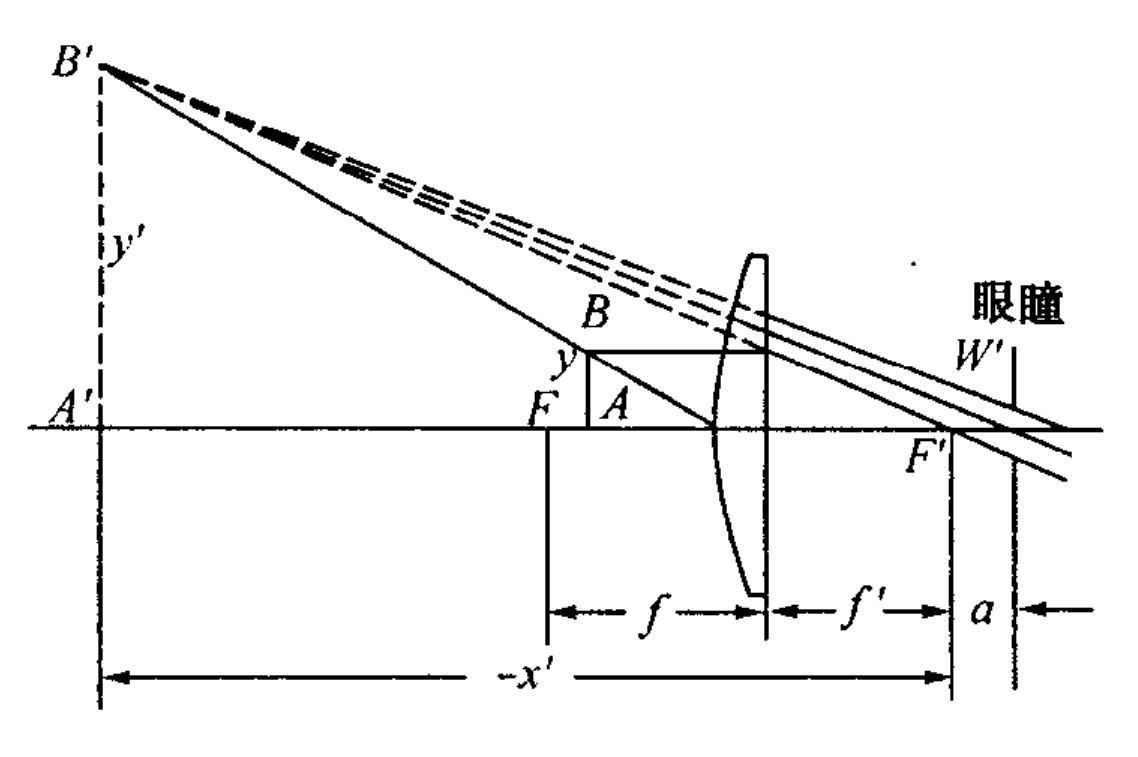
\includegraphics[width=1\textwidth]{magnifier-1.png}
		\caption{放大镜成像示意图}
		\label{fig:magnifier-1}
	\end{minipage}
	\quad
	\begin{minipage}[t]{0.48\textwidth}
		\centering
		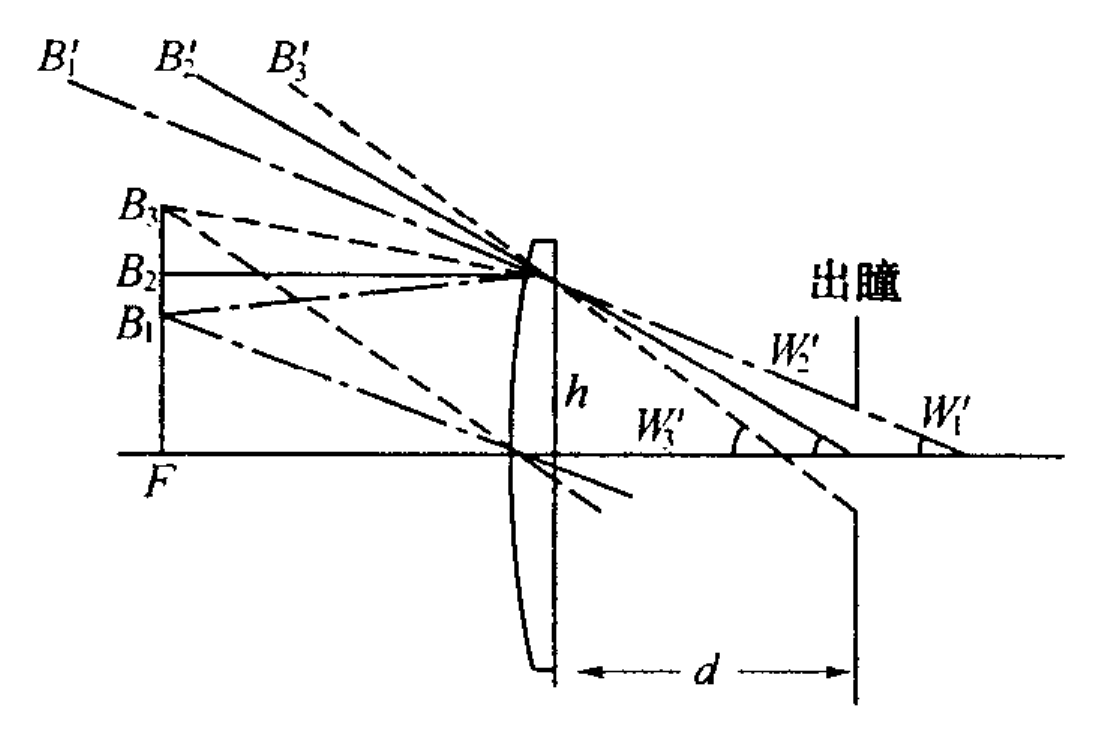
\includegraphics[width=1\textwidth]{magnifier-2.png}
		\caption{放大镜的渐晕}
		\label{fig:magnifier-2}
	\end{minipage}
\end{figure}

如\figref{fig:magnifier-1} 所示,放大镜将位于焦点以内的物$AB$在镜前明视距离处形成虚像$A'B'$,它对眼睛的张角为$W'$,有
\begin{equation}
\tan W'=\frac{y'}{-x'+a}
\end{equation}
而当眼睛直接于明视距离$250\mathrm{mm}$处观察物体时,对眼的张角为$W$,有
\begin{equation}
\tan W=\frac{y}{250}
\end{equation}
以$\tan W'/\tan W$表示放大镜的放大率$M$,并以$\beta=-x'/f'$代替$y'/y$,得
\begin{equation}
M=\frac{250}{f'}\frac{x'}{x'-a}
\end{equation}
由上式可见,放大镜的放大率除与焦距有关外,还与眼睛的位置有关,由于使用放大镜时,眼睛总位于像方焦点附近,$\alpha$相对于$x'$是一小量,于是
\begin{equation}
M=\frac{250}{f'}
\end{equation}
即放大镜的放大率仅由其焦距决定。焦距越短,放大率越大。

一般放大镜的直径比瞳孔直径大得多,物面上各点的成像光束是被眼瞳所限制的。眼瞳是孔径光阑,也是出瞳,放大镜是渐晕光阑。由于放大镜通光口径的限制,视场外围有渐晕而无明晰的边界。\figref{fig:magnifier-2} 画出了决定无渐晕成像范围的$B_1$点、$50\%$渐晕的$B_2$点和可能成像的最边缘点$B_3$,对应视场角分别为$W'_1$、$W'_2$和$W'_3$。由图可见
\begin{equation}
\tan W'_2=\frac{h}{d}
\end{equation}
同理易得出$\tan W'_1$和$\tan W'_3$的表达式。可见,放大镜的直径$2h$越大,眼睛越靠近放大镜,可见的视场就越大。如果以$50\%$渐晕点为界决定线视场,可导出
\begin{equation}
2y=\frac{500h}{Md}
\end{equation}
所以在放大镜的直径可眼瞳位置一定时,放大率越大,线视场越小。这就限制了放大镜的分辨率不能做得很大,一般不超过$15$倍。

\section{显微镜系统}
\label{sect:microscope}
\subsection{显微镜概述}
显微镜的主光学系统由物镜和目镜两部分组成。\figref{fig:microscope-1} 为显微镜的成像原理图。显微镜的总放大率为物镜放大率$M_o$和目镜放大率$M_e$的乘积。这里
\begin{equation}
M_o=\beta=-\frac{\varDelta}{f'_o},\quad M_e=\frac{250}{f'_e}
\end{equation}
即
\begin{equation}
M=M_oM_e=-\frac{250\varDelta}{f'_of'_e}
\end{equation}
式中,$\varDelta=F'_oF_e$,为\textbf{光学筒长}。由此可见,显微镜的放大率与光学筒长成正比,与物镜和目镜的焦距成反比,且$M<0$,即对物体成倒像。

\begin{figure}[htbp]
	\centering
	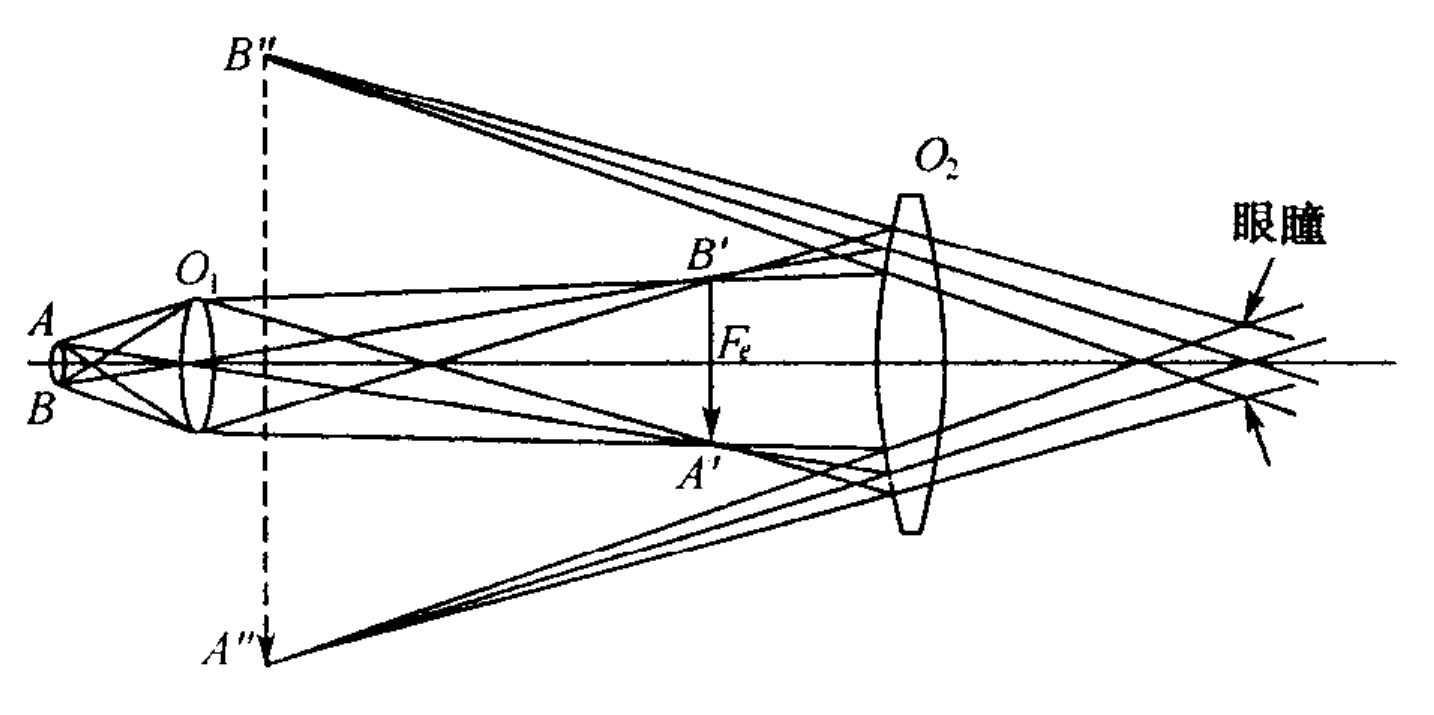
\includegraphics[width=0.6\textwidth]{microscope-1.png}
	\caption{显微镜成像原理图}
	\label{fig:microscope-1}
\end{figure}

\begin{definition}{机械筒长}{mechanical-tube-length}
	显微镜物镜和目镜的支撑面之间的距离$t_m$称为显微镜的机械筒长。我国标准为$160\mathrm{mm}$。
\end{definition}

\subsection{显微镜的孔径光阑}
对于单组低倍显微物镜,其镜框就是孔径光阑;对于多组透镜组成的复杂物镜,或以最后一组的透镜框作为孔径光阑,或在物镜的像方焦面上或其附近专设孔阑。这些孔阑的位置差异相对于光学筒长$\varDelta$是一个小量,因此孔阑被目镜所成的像,即显微镜的出射光瞳都在目镜的像方焦点之外近乎相同的地方,即距目镜像方焦点为$x'=f'^2_e/\varDelta$处。这正是整个显微镜的像方焦面位置。所以,在观察时眼瞳能与出瞳重合,且在更换物镜时不需要改变眼瞳的位置。

\begin{figure}[htbp]
	\centering
	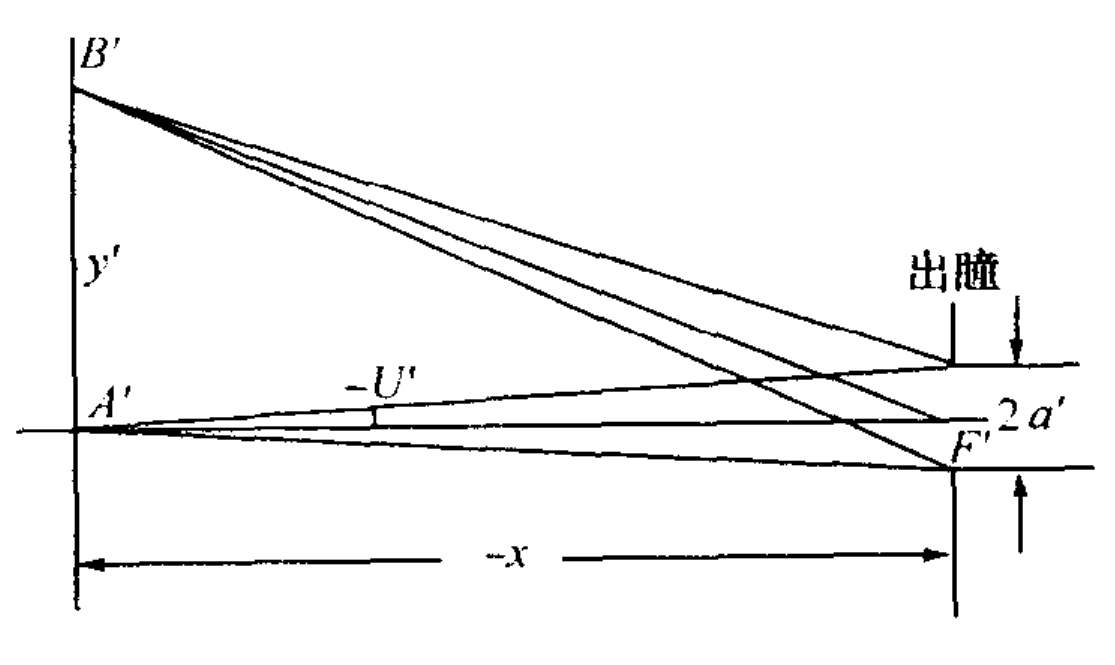
\includegraphics[width=0.6\textwidth]{microscope-2.png}
	\caption{显微镜像方成像}
	\label{fig:microscope-2}
\end{figure}

\figref{fig:microscope-2} 所示的是显微镜像方的成像光束,据此可以求出出瞳的大小为
\begin{equation}
a'=x'\tan U'\approx x'\sin U'
\end{equation}
利用正弦条件$n'y'\sin U'=ny\sin U$和横向放大率$\beta$的表达式,考虑到$n'=1$,可导出
\begin{equation}
a'=-f'n\sin U=-f'A
\end{equation}
式中,$A=n\sin U$称为显微镜物镜的\textbf{数值孔径},是显微镜的一个重要性能参数。引入显微镜的放大率,可得
\begin{equation}
a'=250\frac{A}{M}
\end{equation}
由此可见,显微镜的出瞳主要被其焦距或放大率所决定。高倍率时出瞳很小。

\subsection{显微镜的视场光阑}
在显微镜中间实像平面上有专设的视场光阑,其大小是物面上的可见范围(线视场)与物镜放大率的乘积。因此,高倍物镜只能看到物面上很小的范围,低倍物镜才有较大的视场。

\subsection{显微镜的景深}

\begin{figure}[htbp]
	\centering
	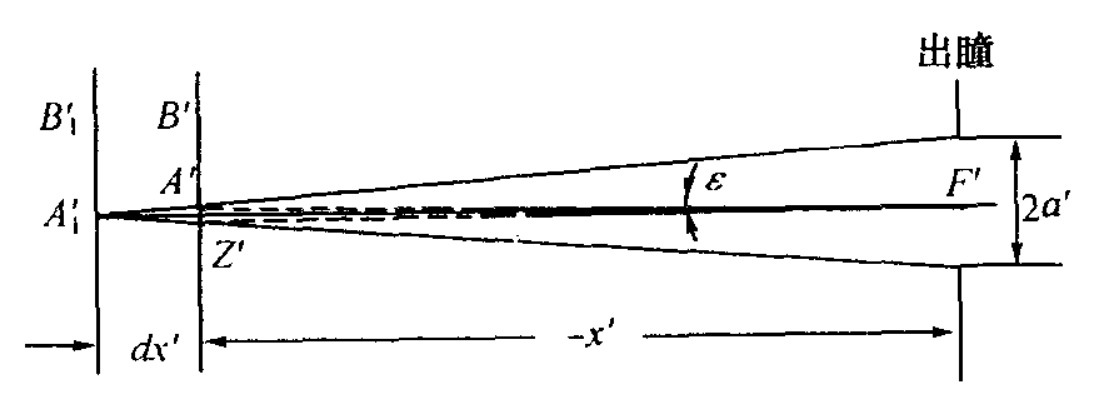
\includegraphics[width=0.6\textwidth]{microscope-depth-of-field.png}
	\caption{显微镜的景深}
	\label{fig:microscope-depth-of-field}
\end{figure}

如\figref{fig:microscope-depth-of-field} 所示,$A'B'$是对准平面被显微镜所成的像,即景像平面,$A'_1B'_1$是对准平面之前的物平面的像,与景深平面相距$\mathrm{d}x'$。设显微镜的出瞳与像方焦面重合,则$A'_1$点的成像光束被景深平面截得一弥散圆,其直径$Z'$由下式决定:
\begin{equation}
\frac{Z'}{2a'}=\frac{\mathrm{d}x'}{-x'+\mathrm{d}x'}
\end{equation}
若弥散圆对出瞳中心的张角不大于眼睛的极限分辨率$\varepsilon$,眼睛观察弥散圆即为点像。此时$2\mathrm{d}x'$即为像方能同时看清景象平面前后两像平面间的深度。因为有$|\mathrm{d}x'|\ll|x'|$,可以得到$2\mathrm{d}x$的表达式。再利用轴向放大率$\alpha=n'\beta^2/n$,将此换算到物方,可得
\begin{equation}
2\mathrm{d}x=\frac{2\mathrm{d}x'}{\alpha}=\frac{nf'^2\varepsilon}{a'}
\end{equation}
再根据$a'=250A/M$以及$M=250/f'$,上式可表示为
\begin{equation}
2\mathrm{d}x=\frac{250n\varepsilon}{MA}
\end{equation}
\begin{property}
由上式可知,显微镜的倍率越高,物镜的数值孔径越大,景深就越小。
\end{property}

由于眼睛能在近点和远点间自行调节,景深将有所扩大。若在像空间中,近点和远点到眼瞳所在的出瞳面的距离为$p'$和$r'$,根据出瞳与显微镜的像方焦面重合可导出与此对应的物空间距离$p$和$r$,两者之差即为眼睛通过显微镜观察时的调节范围,有
\begin{equation}
r=\frac{ff'}{r'}=-\frac{nf'^2}{r'},\quad p=-\frac{nf'^2}{p'}
\end{equation}
\begin{equation}
r-p=-nf'^2\bigg(\frac{1}{r'}-\frac{1}{p'}\bigg)
\end{equation}
当$p'$和$r'$以米为单位时,括号内的值即为眼睛的调节范围$A$,单位为屈光度,即
\begin{equation}
r-p=-0.001nf'^2\overline{A}=-0.001n\overline{A}\bigg(\frac{250}{M}\bigg)^2\Rightarrow r-p\propto\frac{1}{M^2}
\end{equation}
根据以上分析,可以得出显微镜的总景深为$2\mathrm{d}x+(r-p)$。

\subsection{显微镜的分辨率}

\begin{figure}[htbp]
	\centering
	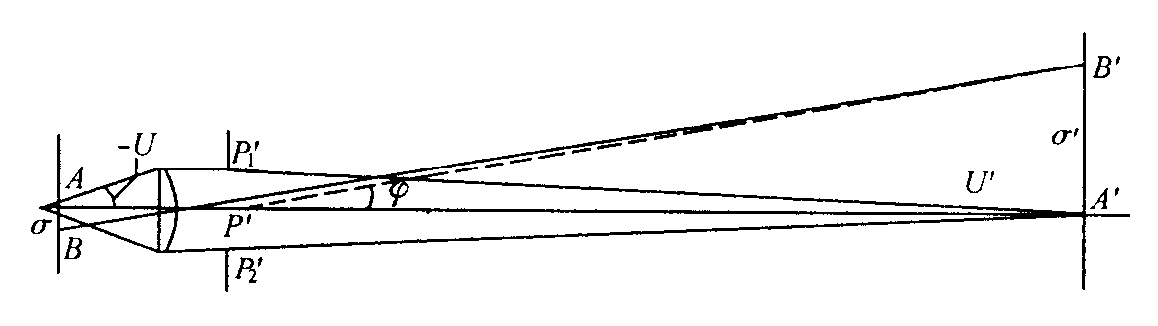
\includegraphics[width=0.8\textwidth]{resolution-of-microscope.png}
	\caption{显微镜分辨不同位置的两点}
	\label{fig:resolution-of-microscope}
\end{figure}

由瑞利判据可知,一个点的衍射像中心正好与另一点的衍射像第一暗环重合时,是光学系统刚好能分辨开这两点的最小界限。从波动光学的原理可知,自身发光的点被理想系统所成的衍射像,其第一暗环半径对出瞳中心所张的角,即正好能被此系统分辨得开的两个点的极限分辨角$\varphi$由式(\ref{eq:limiting-angle-of-resolution})决定,即$\varphi=1.22\lambda/D$。显微镜的分辨率以物面上能被物镜分辨开的两点之间的最小距离表示。如\figref{fig:resolution-of-microscope} 所示,对应的两像点之间的距离$\sigma'$应等于其中任一个衍射斑的第一暗环的半径,又因为像方孔径角很小,有
\begin{equation}
\sigma'=\varphi\cdot P'A'=\frac{0.61\lambda}{\tan U'}=\frac{0.61\lambda}{\sin U'}
\end{equation}

由于显微物镜满足正弦条件$n'\sigma'\sin U'=n\sigma\sin U$,且$n'=1$,所以得到最小分辨距为
\begin{equation}
\sigma=\frac{0.61\lambda}{n\sin U}=\frac{0.61\lambda}{A}
\end{equation}
对物体作斜照明,最小分辨角为
\begin{equation}
\sigma=\frac{0.5\lambda}{n\sin U}
\end{equation}
通过上述讨论可知,对于一定波长的色光,显微镜的分辨率在像差校正良好的情况下,完全被物镜的数值孔径所决定。数值孔径越大,分辨率越高。
\begin{property}
	显微镜的分辨本领随波长的减小而提高,随数值孔径的增大而提高。
\end{property}

\subsection{显微镜的放大率}
分别取$2'$和$4'$为人眼分辨角的下限和上限,人眼在明视距离处能分辨开两点的间距即为$\sigma$被显微镜放大以后的像,有
\begin{equation}
250\times2\times0.00029<\frac{0.5\lambda}{A}M<250\times4\times0.00029
\end{equation}
对于目视光学仪器,主色光波长为$0.00055\mathrm{mm}$,则
\begin{equation}
500A<M<1000A
\end{equation}
满足此公式的放大率称为显微镜的\textbf{有效放大率}。有效放大率由物镜的数值孔径决定,即数值孔径需与放大率相匹配。

\subsection{显微镜的物镜}

显微物镜有折射式、反射式和折反射式三类,绝大多数实用的物镜是折射式。折射式显微物镜可根据质量要求的不同而有不同的类型。
\begin{enumerate}
	\item 消色差物镜
	\begin{enumerate}
		\item 单组双胶合低倍物镜
		\item 李斯特型中倍物镜
		\item 阿米西型高倍物镜
		\item 阿贝浸液物镜
	\end{enumerate}
	\item 复消色差物镜
	\item 平场消色差物镜和平场复消色差物镜
\end{enumerate}

\subsection{显微镜的目镜}
显微镜中目镜相当于放大镜。\textbf{镜目距}是指目镜的出瞳到目镜最后一面的距离,为使眼瞳能和出瞳重合,镜目距不应小于$6\sim8\mathrm{mm}$。在目镜的物方焦面上设置视场光阑,其到目镜第一面的距离称谓目镜的\textbf{工作距离}。显微镜的目镜主要有:惠更斯目镜、冉斯登目镜、补偿目镜、平场目镜。

\subsection{显微镜的照明系统}
显微镜的照明系统主要有以下三类:
\begin{enumerate}
	\item \textbf{用透射光照明透明标本的照明系统:}
	\begin{enumerate}
		\item \textbf{临界照明:}
		
		\begin{figure}[htbp]
			\centering
			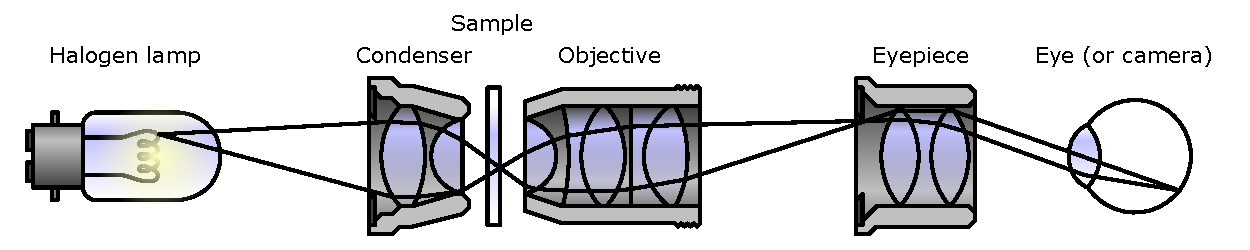
\includegraphics[width=0.9\textwidth]{critical-illumination.pdf}
			\caption{临界照明示意图}
			\label{fig:critical-illumination}
		\end{figure}
		
		光源通过照明系统或聚光镜成像于物面上,如\figref{fig:critical-illumination} 所示。其简化图如图所示(简化图待补充),图中的双点划线是从光源到物面再到像面的一对共轭关系,虚线是从光源光阑到物镜孔阑的另一对共轭关系。聚光镜的像方孔径角必须与物镜的物方孔径角相匹配,为此在聚光镜的物方焦面上或附近设置可变光阑。于是照明系统的出瞳正好与物镜的入瞳大致重合。
		\begin{note}
			临界照明的缺点是当光源的亮度不均匀或呈现明显的灯丝结构时,将会反映到物面上影响观察效果。
		\end{note}
		\item \textbf{柯拉照明:}
		
		\begin{figure}[htbp]
			\centering
			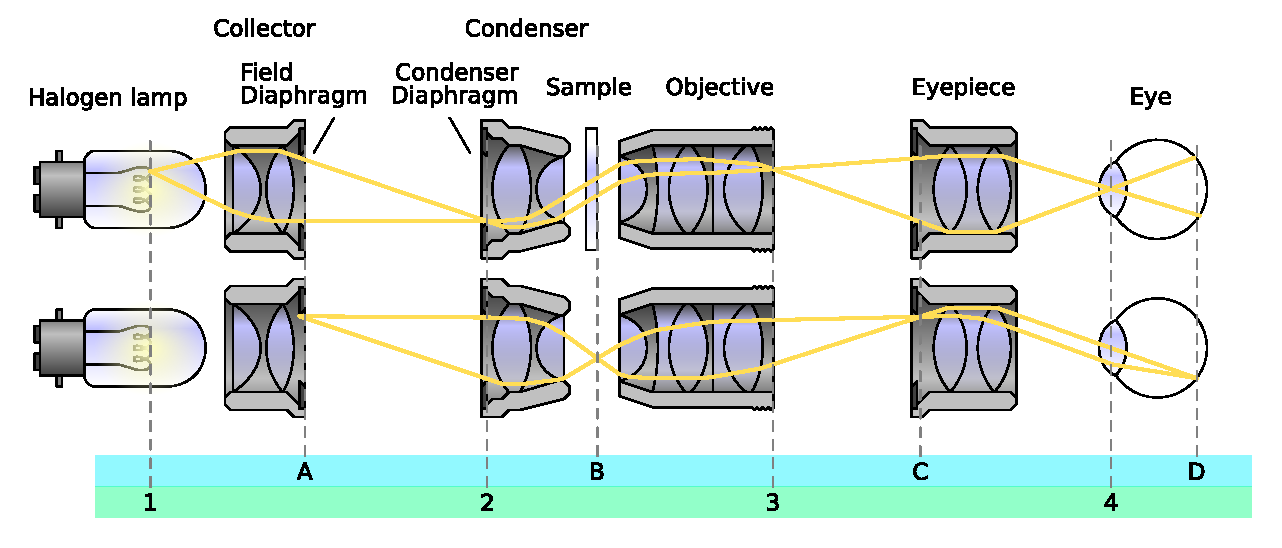
\includegraphics[width=0.9\textwidth]{kohler-illumination.pdf}
			\caption{柯拉照明示意图}
			\label{fig:kohler-illumination}
		\end{figure}
		
		光源成像在物镜入瞳面上,如\figref{fig:kohler-illumination} 所示。图中$A$、$B$、$C$、$D$是一组共轭关系,$1$、$2$、$3$、$4$是一组共轭关系。其简化图如图所示(简化图待补充),图中的虚线是从光源到物镜孔阑的一对共轭关系,双点划线是从光源光阑$J_1$到物面再到像面的另一对共轭关系。光源发出的光先经过一个前置透镜$L$成像于聚光镜前的可变光阑$J_2$上,聚光镜再将此光源像成在物镜的入瞳面上。在前置透镜后紧靠透镜处设置另一可变光阑,它被照明后具有均匀的亮度,并被聚光镜成像于物面上,使物面也得到均匀照明。调节光阑$J_2$可以使照明系统与不同数值孔径的物镜相匹配。调节光阑$J_1$可改变物面上的照明范围。
		\begin{note}
			对比两种照明方式可以发现,柯拉照明可以是临界照明将光源换成光源加前置物镜和光源光阑$J_1$,将光源通过前置物镜成像到$J_2$,$J_1$位于原临界照明的光源位置。
		\end{note}
		\begin{property}
			在照明系统和成像系统的合成系统中,成像系统的所有光都必然来自照明系统。这些光想要到达像面,必须通过照明系统和成像系统各自的瞳和窗。要使光传输的信息量不损失,任一光线都不能被照明系统或成像系统的任一光孔所拦截。那么只可能存在两种光瞳匹配关系,\uline{一种是照明系统的窗与成像系统的窗共轭,照明系统的瞳与成像系统的瞳共轭,这就是临界照明;另一种是照明系统的窗与成像系统的瞳共轭,照明系统的瞳与成像系统的窗共轭,这就是柯拉照明}。
		\end{property}
	\end{enumerate}
	\item \textbf{非透明物体的照明系统:}
	
	光必须从侧面或者正面照明。
	\item \textbf{用暗视场观察微小质点的照明方法:}
	
	用暗视场方法可以观察到超显微质点,即小于显微镜分辨极限的质点。
\end{enumerate}

\section{望远镜系统}
\label{sect:telescope}
\subsection{望远镜的一般特性}
望远镜系统是一种使入射的平行光束仍保持平行射出的光学系统。最简单的望远镜系统必须由两个光组组成。前一光组的像方焦点与后一光组的物方焦点重合,即光学间隔$\varDelta=0$。光组$L_1$朝向物体,为望远镜的物镜;光组$L_2$为目镜。具有正光焦度目镜的系统为\textbf{开普勒望远镜},具有负光焦度目镜的系统为\textbf{伽利略望远镜}。

\begin{figure}[htbp]
	\centering
	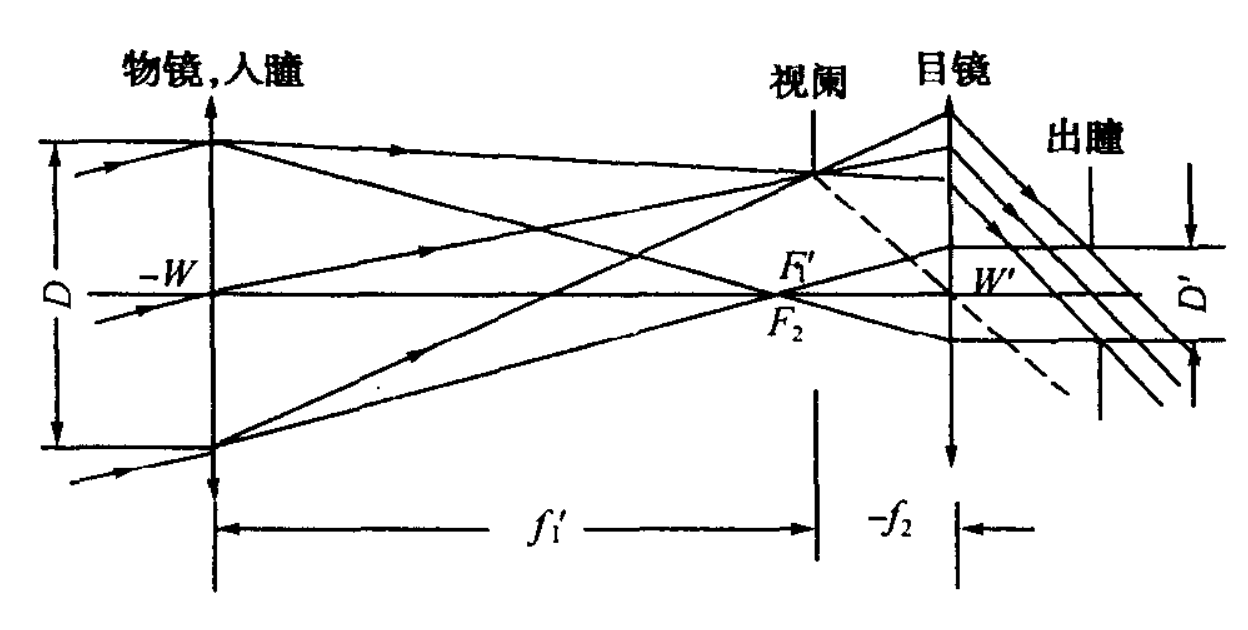
\includegraphics[width=0.7\textwidth]{kepler-telescope.png}
	\caption{开普勒望远镜系统}
	\label{fig:kepler-telescope}
\end{figure}

如\figref{fig:kepler-telescope} 所示为光束经开普勒望远镜系统的光路,物镜的通光孔径限制了轴上点的成像光束,是系统的孔径光阑和入瞳,出瞳是物镜的通光孔被目镜所成的像,应在目镜的像方焦点之外,能与观察者的眼瞳重合。

\begin{definition}{望远镜的放大率}{magnification-of-telescope}
	眼睛通过望远镜观察时,物体的像对眼睛张角的正切与眼睛直接看该物体时,物体对眼睛张角的正切之比,即为望远镜的放大率,以$\varGamma$表示。由于物方、像方都位于无穷远,此放大率即为系统本身的像方视场角与物方视场角的正切值比,有
	\begin{equation}
	\varGamma=\frac{\tan W'}{\tan W}=-\frac{f'_1}{f'_2}=\frac{D}{D'}
	\label{eq:visual-magnification}
	\end{equation}
	所以,望远镜的放大率还可表示为物镜焦距与目镜焦距之比、入瞳直径与出瞳直径之比。由式(\ref{eq:visual-magnification})可知,开普勒望远镜成倒像,伽利略望远镜成正像。
\end{definition}

\begin{property}
由视觉放大率公式(\ref{eq:visual-magnification})可知:
\begin{enumerate}
	\item 当物镜的焦距大于目镜的焦距时,望远镜有视觉放大作用;
	\item 当目镜的焦距一定时,倍率越高,物镜的焦距越长,导致望远镜的长度越大;
	\item 当像方视场角$W'$一定时,倍率越大,物方视场越小;
	\item 当入瞳直径一定时,倍率越大,出瞳直径越小,当出瞳小于眼瞳时,视见像的光强度下降。
\end{enumerate}
\end{property}

\begin{definition}{望远镜的正常放大率}{normal-magnification-of-telescope}
	当望远镜的入瞳直径为$D$时,它能分辨的远处两点对入瞳中心的最小张角为$\varphi''=140/D$,为充分利用物镜的分辨率,望远镜应把此角度放大到能为眼睛所分辨的程度,因此要求$\varGamma\varphi''\geqslant60''\sim70''$,即
	\begin{equation}
	\varGamma\geqslant0.5D
	\end{equation}
	式中,$D$的单位为毫米。按照此式确定的放大率称为望远镜的正常放大率,对应的出瞳直径为$2\mathrm{mm}$,和白天光亮条件下眼瞳直径相当。
\end{definition}
较多情况下按仪器用途确定的放大率大于正常放大率。若通过望远镜瞄准,则瞄准误差应为
\begin{equation}
\Delta\alpha''=\frac{\alpha''}{\varGamma}
\end{equation}
式中$\alpha''$为肉眼瞄准误差,由此可见增大倍率可提高瞄准镜度。

\subsection{望远镜的主观亮度}
\begin{definition}{主观亮度}{subjective-luminance}
	眼睛观物时,成在视网膜上的像对感光神经末梢的作用所引起的视觉刺激程度,称为主观亮度。眼睛直接观物时感知的像的明亮程度称为肉眼的主观亮度;通过望远镜观察时感知的像的明亮程度称为望远镜的主观亮度。
\end{definition}

\subsubsection{点物或点光源的像}
	
像的主观亮度仅决定于进入眼睛的光通量。当通过望远镜观察点光源时,能进入望远镜的光通量$\varPhi_T$被入瞳直径$D$决定,用人眼直接观察时,能进入眼瞳的光通量$\varPhi_e$由眼瞳的直径$D_e$决定。若眼瞳直径$D_e$大于望远镜的出瞳直径$D'$,所有射入望远镜的光通量全部都能进入眼睛,因此点像的主观亮度要比肉眼观察时大。其相对主观亮度,即两种情况下的光通量之比为:
\begin{equation}
\frac{\varPhi_T}{\varPhi_e}=k\frac{D^2}{D^2_e}
\label{eq:relative-subjective-luminance-1}
\end{equation}
其中,$k$为望远镜的透射率。若望远镜的出瞳直径$D'$与眼瞳直径$D_e$相等,此时有$D=\varGamma D_e$,则相对主观亮度为
\begin{equation}
\frac{\varPhi_T}{\varPhi_e}=k\varGamma^2
\label{eq:relative-subjective-luminance-2}
\end{equation}
若出瞳大于眼瞳,则进入望远镜的光通量不能全部进入眼瞳,眼睛便成为整个光学系统的出瞳,入瞳直径应为$\varGamma D_e$,此时同样可得公式(\ref{eq:relative-subjective-luminance-2})。
\begin{property}
	望远镜的物镜口径一定时,倍率越高,相对主观亮度越大,但倍率高到使出瞳不大于眼瞳时,即为定值。当望远镜的倍率和眼瞳直径一定时,物镜的直径越大,相对主观亮度也越大。
\end{property}
观察天空中微弱发光的星星时,应使用倍率高,物镜孔径大的天文望远镜。
	
\subsubsection{观察有限大小物体}
	
有限大小物体的像的主观亮度由网膜上的照度决定。通过望远镜观察的物体与人眼直接观察同一物体在视网膜上像面积之比为$\varGamma^2$,由$E=\varPhi/S$与式(\ref{eq:relative-subjective-luminance-1})可得观察有限大小物体的相对主观亮度为
\begin{equation}
\frac{E_T}{E_e}=k\bigg(\frac{D'}{D_e}\bigg)^2
\end{equation}
上式的值不可能大于$k$,因此用望远镜观察有限大小的物体时,主观亮度总比用肉眼观察时低。所以在黄昏或夜间使用的望远镜因眼瞳较大,应有较大的出瞳。望远镜的倍率越高,出瞳越小,当用于天文观察时,作为点光源的星星,其相对主观亮度很大,而作为背景的天空,相对主观亮度很小,因此在白天,利用高倍天文望远镜可以看见明亮天空中的星星。

\subsection{望远镜的光束限制}

伽利略望远镜和开普勒望远镜具有不同的光束限制。

\figref{fig:galileo-telescope} 所示的是伽利略望远镜物方的入瞳和物镜、像方的出瞳和渐晕光阑的像。根据几何关系可以得出无渐晕、$50\%$渐晕的视场角,后者的正切为
\begin{equation}
\tan W=\frac{D}{2l}=\frac{D}{2\varGamma(f'_1+f'_2+\varGamma l'_p)}
\end{equation}
式中,$D$为物镜的直径,$l'_p$为出瞳距。由此可见,伽利略望远镜的倍率越高,视场越小,视场还随眼睛远离目镜而变小。
\begin{figure}[htbp]
	\centering
	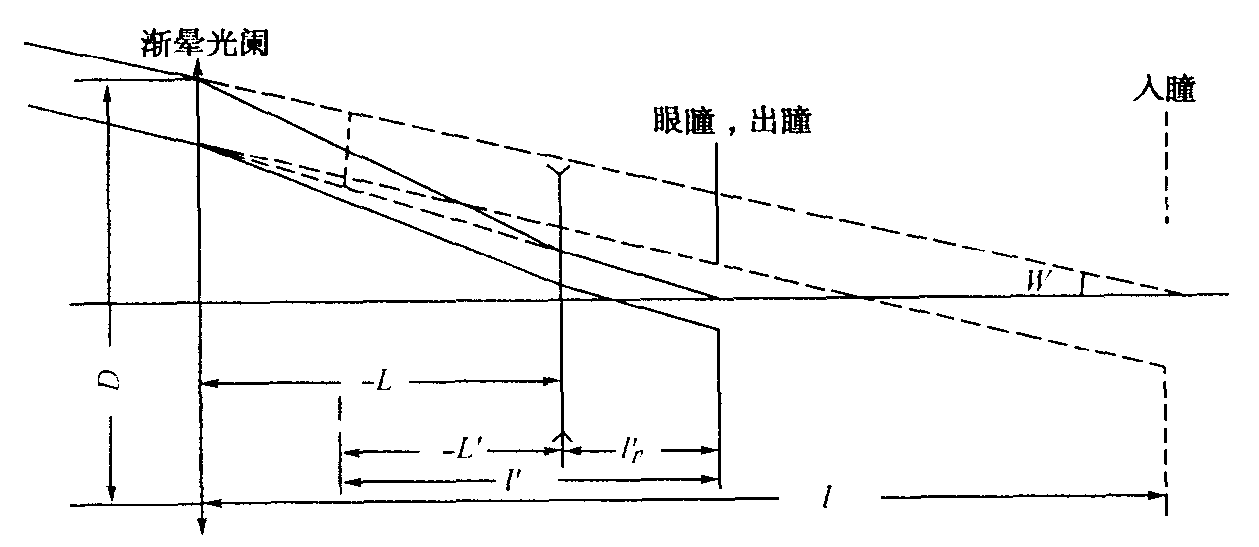
\includegraphics[width=0.8\textwidth]{galileo-telescope.png}
	\caption{伽利略望远镜系统}
	\label{fig:galileo-telescope}
\end{figure}
\begin{note}
	伽利略望远镜的优劣:伽利略望远镜的优点在于结构简单,筒长短,轻便,光能损失少,成正像。但伽利略望远镜没有中间的实像面,不能设置分划板作瞄准和定位。	
\end{note}

开普勒望远镜的目镜为正光焦度,在物镜和目镜之间具有中间实像平面,可以在其上设置视阑,安装分划板,作瞄准、定位和测量之用。分划板是在磨光的玻璃片上刻以分划标志的光学零件,其通光口径就是视阑的直径,有
\begin{equation}
D_F=2f'\tan W
\end{equation}
通过开普勒望远镜观察物体时,有明晰的视场边界。为了在大相对孔径和大视场的情况下不致使目镜的直径太大,并减少目镜斜光束像差的有害影响,可适当减小目镜的口径而允许轴外点存在$50\%$的渐晕。此时\figref{fig:kepler-telescope} 中主光线以上部分光束将被目镜限制而不能通过。
\begin{note}
	开普勒望远镜成倒像,只适用于天文观测或专设目标的瞄准和测量,为了便于观察可加入转像系统。结构上比伽利略望远镜复杂。	
\end{note}

\subsection{望远镜的物镜}
望远镜物镜只需要对轴上点校正色差、球差和对近轴点校正彗差,轴外像差可不予考虑,其结构比较简单。
\begin{enumerate}
	\item 折射式望远镜物镜:双胶合物镜、双分离物镜、三分离物镜、内调焦物镜
	\item 反射式望远镜物镜:卡塞格林系统、格利果里系统
	\item 折反射式望远镜物镜:施密特物镜、马克苏托夫物镜、无光焦度的双透镜与球面卡氏系统的组合
\end{enumerate}
\begin{note}
	$D>60\mathrm{mm}$时不适于胶合。双分离物镜的$d_{\mathrm{air}}\approx0$。反射式物镜的$D$很大,对材料无严格要求,筒长较短,完全无色差,但对表面质量要求更高,且要用非球面。折反射式物镜以球面反射镜为基础,再加用于校正像差的折射元件而构成,可避免大型非球面加工。
\end{note}
\subsection{望远镜的目镜}
用于瞄准和测量的望远镜在其视阑平面上设置有分划板。为使屈光不正的观察者能看清分划板,目镜应能做视度调节。设调节量为$\Delta l$,则
\begin{equation}
\Delta lx'=xx'=f_2f'_2
\end{equation}
其中,$x'$为远点距。若要求视度的调节范围为$\pm N$个屈光度,目镜相对于分划板的调焦量$\Delta l$应为
\begin{equation}
\Delta l=\pm\frac{Nf'^2_2}{1000}(\mathrm{mm})
\end{equation}
式中,$f'_2$为目镜的焦距,以毫米计,一般仪器中,要求$N=\pm5$屈光度。目镜的工作距离应大于$\Delta l$。常用的目镜有:冉斯登目镜、凯涅尔目镜、对称式目镜、阿贝无畸变目镜、爱弗尔目镜。
\begin{note}
	工作距离不等于焦距。
\end{note}
\begin{property}
	望远镜物镜与目镜的参数比较:
	\begin{itemize}
		\item 物镜:$f'$大,$D/f'$中等,$2W$小;
		\item 目镜:$f'$小,$D/f'$中等,$2W$大。
	\end{itemize} 	
\end{property}

\subsection{转像系统与场镜}
实际应用中使用的望远镜都是利用转像系统使倒像转成正像的开普勒望远镜。这种望远镜称为地上望远镜,转像系统为棱镜系统或透镜系统。
\subsubsection{棱镜转像系统}
用单块屋脊棱镜或由普通棱镜组合起来的棱镜系统,均能达到使像相对于物体在上下和左右两个方向都倒转过来的目的。详见第 \ref{sect:reflecting-prism} 节。

\subsubsection{透镜转像系统}
\begin{definition}{透镜转像系统}{lens-steering-system}
	设在物镜的实像平面后面,使倒像再一次倒转成为正像的透镜系统称为透镜转像系统。
\end{definition}
透镜转像系统有两种形式,如\figref{fig:lens-steering-system-1} 和\figref{fig:lens-steering-system-2} 所示。

\begin{figure}[htbp]
	\centering
	\begin{tikzpicture} 
	\draw[-] (-5,0) -- (5,0);
	\draw[latex-latex] (-4,1.2) -- (-4,-1.2);
	\draw[-latex] (-1.75,0.8) -- (-1.75,-0.8);
	\draw[latex-latex] (0.5,1.2) -- (0.5,-1.2);
	\draw[latex-] (2.825,0.8) -- (2.825,-0.8);
	\draw[latex-latex] (4,1) -- (4,-1);
	\draw[-] (-5,1) -- (-4,1);
	\draw[-] (-4,1) -- (0.5,-1);
	\draw[-] (4,0.5) -- (0.5,-1);
	\draw[-] (4,0.5) -- (5,0.5);
	\draw[-] (-5,-1) -- (-4,-1);
	\draw[-] (-4,-1) -- (0.5,1);
	\draw[-] (4,-0.5) -- (0.5,1);
	\draw[-] (4,-0.5) -- (5,-0.5);
	\node[] at (-4,1.5) {物镜};
	\node[] at (-1.75,1.1) {中间像};
	\node[] at (0.5,1.5) {转像透镜};
	\node[] at (2.825,1.1) {视阑};
	\node[] at (4,1.3) {目镜};
	\end{tikzpicture}
	\caption{透镜转像系统(单组)}
	\label{fig:lens-steering-system-1}
\end{figure}
\begin{figure}[htbp]
	\centering
	\begin{tikzpicture} 
	\draw[-] (-5,0) -- (7,0);
	\draw[latex-latex] (-4,1.2) -- (-4,-1.2);
	\draw[-latex] (-1.75,0.8) -- (-1.75,-0.8);
	\draw[latex-latex] (0.5,1.2) -- (0.5,-1.2);
	\draw[latex-latex] (2.5,1.2) -- (2.5,-1.2);
	\draw[latex-] (4.825,0.8) -- (4.825,-0.8);
	\draw[latex-latex] (6,1) -- (6,-1);
	\draw[-] (-5,1) -- (-4,1);
	\draw[-] (-4,1) -- (0.5,-1);
	\draw[-] (0.5,-1) -- (2.5,-1);
	\draw[-] (6,0.5) -- (2.5,-1);
	\draw[-] (6,0.5) -- (7,0.5);
	\draw[-] (-5,-1) -- (-4,-1);
	\draw[-] (-4,-1) -- (0.5,1);
	\draw[-] (0.5,1) -- (2.5,1);
	\draw[-] (6,-0.5) -- (2.5,1);
	\draw[-] (6,-0.5) -- (7,-0.5);
	\node[] at (-4,1.5) {物镜};
	\node[] at (-1.75,1.1) {中间像};
	\node[] at (1.5,1.5) {转像透镜};
	\node[] at (4.825,1.1) {视阑};
	\node[] at (6,1.3) {目镜};
	\end{tikzpicture}
	\caption{透镜转像系统(双组)}
	\label{fig:lens-steering-system-2}
\end{figure}
单组透镜转像系统使筒长加长了$4$倍转像透镜焦距的长度,转像透镜的$\beta=-1$;
双组透镜转像系统的镜筒加长
\begin{equation}
L=f'_a+d+f'_b\xrightarrow{f'_a=f'_b}2f'_a+d
\end{equation}
前后两块转像透镜取对称结构使转像组的垂轴像差为零。
\subsubsection{场镜}
\begin{definition}{场镜}{field-lens}
	如果只是简单地加入透镜转像系统,轴外点成像光束在转像镜组上的入射高度会大大增加,导致视场较大,绝大部分光线不能通过转像系统。为此,可以在中间实像平面上加一适当光焦度的透镜,使望远镜的光瞳与转像系统的光瞳共轭,使轴外光束折向转像镜组。这种加于中间相面上或附近的透镜称为场镜。
\end{definition}
加入场镜后,总光焦度
\begin{equation}
\varphi=\frac{1}{h_1}\sum h\varphi
\end{equation}
保持不变,即场镜的光焦度对系统的总光焦度并无贡献,不影响轴上点光束和系统的放大率。

根据像差理论可知,位于像面上的场镜除了产生匹兹凡和以及由此引起的畸变外,不产生其他像差。因此场镜都使用单透镜,并且在不需由它来改变畸变时,都采用平凹透镜。

\subsection{外形尺寸计算}
\begin{problem}
	\textbf{\color{red}{(重点)}}镜筒的长度为$250\mathrm{mm}$、放大率为$-24$、视场角为$1^{\circ}48'$的开普勒望远镜,设入瞳与物镜重合,计算其外形尺寸。
\end{problem}
\begin{solution}
	镜筒长度为$250\mathrm{mm}$,放大率为$-24$,有
	\begin{equation}
	f'_1+f'_2=250\mathrm{mm},\quad \varGamma=-\frac{f'_1}{f'_2}=-24 \nonumber
	\end{equation}
	所以,$f'_1=240\mathrm{mm}$,$f'_2=10\mathrm{mm}$。由于正常放大率$\varGamma=0.5D$,则入瞳直径为$D=48\mathrm{mm}$,根据公式
	\begin{equation}
	\varGamma=\frac{D}{D'} \nonumber
	\end{equation}
	得到出瞳直径为$D'=2\mathrm{mm}$。根据公式
	\begin{equation}
	D_F=2f'_1\tan W \nonumber
	\end{equation}
	得到视阑直径为$D_F=7.54\mathrm{mm}$,取$D_F=7.6\mathrm{mm}$。由于视场角为$1^{\circ}48'$,根据公式
	\begin{equation}
	\varGamma=\frac{\tan W'}{\tan W} \nonumber
	\end{equation}
	得到目镜视场(即像方视场角)为$2W'=41.32^{\circ}$。根据公式
	\begin{equation}
	l'_p=x'_p+f'_2=\frac{f_2f'_2}{-f'_1}+f'_2=-\frac{L}{\varGamma} \nonumber
	\end{equation}
	得到出瞳距为$l'_p=10.42\mathrm{mm}$。目镜的通光口径与渐晕系数有关,无渐晕时,根据公式
	\begin{equation}
	\frac{D_e-D'}{2l'_p}=\tan W' \nonumber
	\end{equation}
	得到目镜直径为$D_e=9.86\mathrm{mm}$。若要求目镜的视度调节为$\pm5$屈光度,根据公式
	\begin{equation}
	\Delta l=\pm\frac{Nf'^2_2}{1000}(\mathrm{mm}) \nonumber
	\end{equation}
	得调节距离为$\Delta l=\pm0.5\mathrm{mm}$。
\end{solution}